%
% Template for RBIE papers in LaTeX
%

% The above language combination is for this template document only.
% You should use one of the following:
\documentclass[english, spanish, brazilian]{RBIEarticle} % for papers in portuguese
%\documentclass[brazilian, spanish, english]{RBIEarticle} % for papers in english
%\documentclass[brazilian, english, spanish]{RBIEarticle} % for papers in spanish

% Papers in Portuguese or Spanish may require the following lines:
\usepackage[utf8]{inputenc} % chooses UTF-8 as the main character set
\usepackage[T1]{fontenc} % for correct syllable separation in accented words

% The next two statements are needed for the example table in this document
% (i.e. you don't necessarily need them in your own paper)
\usepackage{colortbl}
\definecolor{gray}{gray}{.8}

% Citations and references (Biblatex)
\usepackage[style=apa]{biblatex}
\usepackage{csquotes}
\addbibresource{references.bib}

% Here goes the paper main title
\title{Modelo de Metaprojeto para Integração de Ferramentas e Processos de Avaliação em Project-Based Learning: Abordagem Arquitetural Baseada em Digital Twins}

% If the manuscript is written in English, then this element must be removed.
\titleinenglish{Metaproject Model for Integration of Assessment Tools and Processes in Software Engineering Project-Based Learning: A Digital Twin Architectural Approach}

% If the manuscript is written in English, then this element must be removed.
\titleinspanish{Modelo de Metaproyecto para Integración de Herramientas y Procesos de Evaluación en Project-Based Learning: Enfoque Arquitectónico Basado en Digital Twins}

% Here goes the paper author information (repeat for two or more authors)
\author{%
	\parbox{8cm}{%
		aaaa\\
		aaaa\\
		ORCID: \href{https://orcid.org/0000-0000-0000-0000}{0000-0000-0000-0000}\\
		aaaa@aaaa.com
	}
}

\Submission{dd/Mmm/yyyy}
\First_round_notif{dd/Mmm/yyyy}
\New_version{dd/Mmm/yyyy}
\Second_round_notif{dd/Mmm/yyyy}
\Camera_ready{dd/Mmm/yyyy}
\Edition_review{dd/Mmm/yyyy}
\Available_online{dd/Mmm/yyyy}
\Published{dd/Mmm/yyyy}

% Here goes the page heading information
\heading{aaaa}{RBIE v.VV – yyyy}

% And finally here goes the citation information
\citeas{aaaa (Year). Modelo de Metaprojeto para Integração de Ferramentas e Processos de Avaliação em Project-Based Learning: Abordagem Arquitetural Baseada em Digital Twins. Revista Brasileira de Informática na Educação, vol, pp-pp. https://doi.org/10.5753/rbie.yyyy.id}

%====================================================================
%\hyphenpenalty=10000
%\setcounter{page}{01}

\begin{document}
\maketitle

% If the manuscript is written in English, then this element must be removed.
\begin{otherlanguage}{brazilian}
\begin{abstract}
Este artigo propõe um modelo arquitetural para integração de ferramentas e processos de avaliação em Project-Based Learning (PBL) aplicado ao ensino de engenharia de software. A pesquisa identifica uma lacuna na literatura sobre ferramentas de suporte para docentes na avaliação contínua de projetos educacionais. O modelo proposto utiliza abordagens de modelagem arquitetural (IDF0 e UML) para estruturar o metaprojeto de um módulo PBL, integrando três visões: estrutural, comportamental e de processo. A metodologia Design Science Research foi empregada para desenvolver o modelo conceitual, que serve como base para futuras implementações de digital twins educacionais. O estudo demonstra como a modelagem arquitetural pode apoiar docentes na avaliação multidimensional de artefatos produzidos pelos estudantes durante sprints de desenvolvimento. Os resultados indicam que o modelo oferece uma estrutura conceitual robusta para integração de ferramentas de avaliação, preenchendo uma lacuna identificada na literatura sobre suporte pedagógico em PBL.
\keywords Project-Based Learning; Engenharia de Software; Modelagem Arquitetural; Avaliação Educacional; Digital Twins; Metaprojeto
\end{abstract}
\end{otherlanguage}

\begin{otherlanguage}{english}
\begin{abstract}
This article proposes an architectural model for integrating assessment tools and processes in Project-Based Learning (PBL) applied to software engineering education. The research identifies a gap in the literature regarding support tools for teachers in the continuous assessment of educational projects. The proposed model uses architectural modeling approaches (IDF0 and UML) to structure the metaproject of a PBL module, integrating three views: structural, behavioral, and process. Design Science Research methodology was employed to develop the conceptual model, which serves as a foundation for future implementations of educational digital twins. The study demonstrates how architectural modeling can support teachers in the multidimensional assessment of artifacts produced by students during development sprints. The results indicate that the model provides a robust conceptual structure for integrating assessment tools, filling a gap identified in the literature regarding pedagogical support in PBL.
\keywords Project-Based Learning; Software Engineering; Architectural Modeling; Educational Assessment; Digital Twins; Metaproject
\end{abstract}
\end{otherlanguage}

% If the manuscript is written in English, then this element must be removed.
\begin{otherlanguage}{spanish}
\begin{abstract}
Este artículo propone un modelo arquitectónico para la integración de herramientas y procesos de evaluación en Project-Based Learning (PBL) aplicado a la enseñanza de ingeniería de software. La investigación identifica una brecha en la literatura sobre herramientas de apoyo para docentes en la evaluación continua de proyectos educativos. El modelo propuesto utiliza enfoques de modelado arquitectónico (IDF0 y UML) para estructurar el metaproyecto de un módulo PBL, integrando tres vistas: estructural, comportamental y de proceso. Se empleó la metodología Design Science Research para desarrollar el modelo conceptual, que sirve como base para futuras implementaciones de gemelos digitales educativos. El estudio demuestra cómo el modelado arquitectónico puede apoyar a los docentes en la evaluación multidimensional de artefactos producidos por los estudiantes durante sprints de desarrollo. Los resultados indican que el modelo proporciona una estructura conceptual robusta para la integración de herramientas de evaluación, llenando una brecha identificada en la literatura sobre apoyo pedagógico en PBL.
\keywords Project-Based Learning; Ingeniería de Software; Modelado Arquitectónico; Evaluación Educativa; Digital Twins; Metaproyecto
\end{abstract}
\end{otherlanguage}

\pagebreak

%====================================================================

\section{Introdução}

O ensino de engenharia de software enfrenta desafios significativos na avaliação de competências práticas e técnicas dos estudantes, especialmente em metodologias baseadas em projetos como o Project-Based Learning (PBL). A literatura atual revela uma lacuna importante: a ausência de ferramentas de suporte estruturadas para docentes na avaliação contínua e multidimensional de artefatos produzidos durante o desenvolvimento de projetos educacionais.

O PBL em engenharia de software apresenta características únicas que demandam abordagens de avaliação específicas. Os estudantes trabalham em equipes, desenvolvem artefatos técnicos complexos (código, documentação, arquitetura), e seguem metodologias ágeis com sprints de desenvolvimento. Esta complexidade torna desafiador para os docentes acompanhar e avaliar adequadamente o progresso e a qualidade dos trabalhos produzidos.

A pesquisa bibliográfica realizada não identificou trabalhos que integrem modelagem arquitetural com ferramentas de suporte para docentes em PBL. Especificamente, não foram encontrados estudos que utilizem abordagens de modelagem como IDF0 (Integrated Definition for Function Modeling) e UML (Unified Modeling Language) para estruturar metaprojetos educacionais que sirvam como base para instrumentos de avaliação pedagógica.

Este artigo propõe um modelo arquitetural conceitual que utiliza técnicas de modelagem para estruturar o metaprojeto de um módulo PBL em engenharia de software. O modelo integra três visões arquiteturais (estrutural, comportamental e de processo) e serve como ferramenta de suporte para docentes na avaliação de artefatos produzidos pelos estudantes durante sprints de desenvolvimento.

A contribuição principal deste trabalho é a proposição de um modelo conceitual que preenche a lacuna identificada na literatura, oferecendo uma estrutura arquitetural que pode ser utilizada como base para futuras implementações de digital twins educacionais, sem comprometer a natureza conceitual da proposta.

\section{Referencial Teórico}

\subsection{Project-Based Learning em Engenharia de Software}

O Project-Based Learning (PBL) tem se consolidado como uma metodologia eficaz para o ensino de engenharia de software, oferecendo aos estudantes experiências práticas que simulam ambientes profissionais reais. Segundo \parencite{Thomas2000}, o PBL caracteriza-se por projetos centrais que organizam e impulsionam o aprendizado, resultando em produtos finais que demonstram a compreensão e aquisição de competências.

No contexto específico da engenharia de software, o PBL apresenta características particulares que o diferenciam de outras áreas. Os projetos envolvem o desenvolvimento de sistemas de software reais, com requisitos complexos, metodologias ágeis, e artefatos técnicos diversos como código-fonte, documentação de arquitetura, testes automatizados, e documentação de usuário.

\subsection{Modelagem Arquitetural em Educação}

A modelagem arquitetural oferece ferramentas conceituais poderosas para estruturar e compreender sistemas complexos. No contexto educacional, estas abordagens podem ser aplicadas para modelar processos de ensino-aprendizagem, estruturas curriculares, e sistemas de avaliação.

O IDF0 (Integrated Definition for Function Modeling) é uma técnica de modelagem que permite representar sistemas através de diagramas hierárquicos de funções. Cada função é definida por suas entradas, saídas, controles e mecanismos, oferecendo uma visão clara dos processos e suas interdependências.

O UML (Unified Modeling Language) fornece notações padronizadas para modelar sistemas de software, incluindo diagramas de classes que representam a estrutura estática do sistema, suas entidades, atributos e relacionamentos.

\subsection{Digital Twins e Educação}

Os digital twins têm emergido como uma tecnologia promissora para diversos domínios, incluindo a educação. Um digital twin é uma representação virtual de um sistema físico que mantém sincronização em tempo real, permitindo monitoramento, análise e simulação.

No contexto educacional, os digital twins podem ser aplicados para criar representações virtuais de ambientes de aprendizagem, processos educacionais, e sistemas de avaliação. Esta abordagem permite aos docentes acompanhar o progresso dos estudantes de forma mais granular e oferecer feedback personalizado.

\subsection{Lacuna Identificada na Literatura}

A revisão bibliográfica realizada identificou uma lacuna significativa: não foram encontrados trabalhos que integrem modelagem arquitetural (IDF0 e UML) com ferramentas de suporte para docentes em PBL de engenharia de software. Especificamente, há carência de abordagens que utilizem modelos conceituais como base para instrumentos de avaliação pedagógica.

Esta lacuna representa uma oportunidade importante para contribuir com a literatura, oferecendo uma proposta metodológica estruturada que pode apoiar docentes na avaliação contínua e multidimensional de projetos educacionais.

\section{Metodologia}

Este trabalho utiliza a metodologia Design Science Research (DSR), que é apropriada para o desenvolvimento de artefatos conceituais e tecnológicos que resolvem problemas práticos. O DSR segue um processo iterativo de design, desenvolvimento e avaliação, permitindo a criação de soluções inovadoras baseadas em fundamentos teóricos sólidos.

O processo de DSR implementado neste trabalho incluiu as seguintes etapas:

\begin{enumerate}
    \item \textbf{Identificação do Problema}: Análise da lacuna na literatura sobre ferramentas de suporte para docentes em PBL
    \item \textbf{Definição dos Objetivos}: Desenvolvimento de um modelo arquitetural conceitual para integração de ferramentas de avaliação
    \item \textbf{Design e Desenvolvimento}: Criação do modelo utilizando técnicas de modelagem IDF0 e UML
    \item \textbf{Demonstração}: Aplicação do modelo em um contexto de PBL em engenharia de software
    \item \textbf{Avaliação}: Análise da adequação do modelo para o problema identificado
\end{enumerate}

A modelagem arquitetural foi realizada utilizando duas técnicas complementares:

\begin{itemize}
    \item \textbf{IDF0}: Para modelar os processos e fluxos do metaprojeto PBL
    \item \textbf{UML - Diagrama de Classes}: Para representar a estrutura estática das entidades e relacionamentos
\end{itemize}

\section{Modelo Proposto}

\subsection{Visão Geral do Modelo}

O modelo proposto estrutura o metaprojeto de um módulo PBL em engenharia de software através de três visões arquiteturais integradas:

\begin{itemize}
    \item \textbf{Visão Estrutural}: Representada pelo diagrama de classes UML, define as entidades, atributos e relacionamentos do sistema educacional
    \item \textbf{Visão Comportamental}: Captura os comportamentos e interações entre as entidades do sistema
    \item \textbf{Visão de Processo}: Modelada através de diagramas IDF0, representa os fluxos de trabalho e processos educacionais
\end{itemize}

\subsection{Modelagem Estrutural - Diagrama de Classes}

O diagrama de classes representa a estrutura estática do metaprojeto PBL, definindo as principais entidades e seus relacionamentos. As classes principais incluem:

\begin{itemize}
    \item \textbf{Módulo}: Representa um módulo PBL com atributos como nome, duração, e objetivos de aprendizagem
    \item \textbf{Projeto}: Representa um projeto específico desenvolvido pelos estudantes
    \item \textbf{Sprint}: Representa uma iteração de desenvolvimento com artefatos associados
    \item \textbf{Artefato}: Representa produtos produzidos pelos estudantes (código, documentação, etc.)
    \item \textbf{Estudante}: Representa os participantes do projeto
    \item \textbf{Docente}: Representa os professores responsáveis pela avaliação
\end{itemize}

\begin{figure}[h]
	\centerline{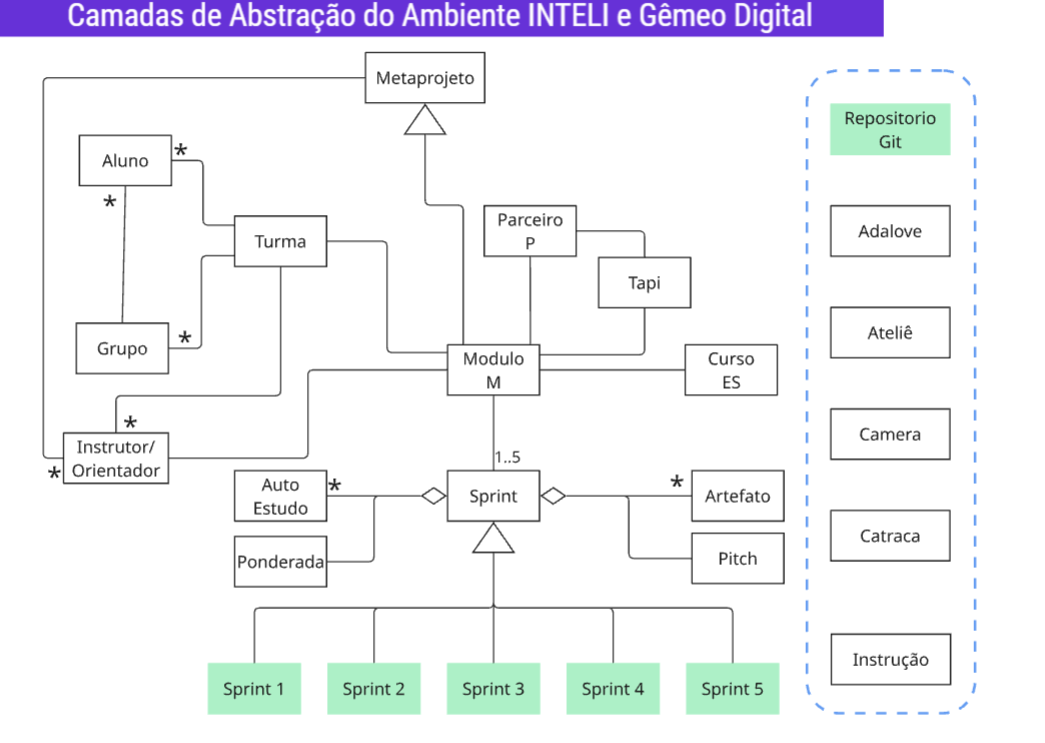
\includegraphics[scale=0.6]{assets/modelo_de_classes.png}}
	\caption{Diagrama de Classes do Metaprojeto PBL}
	\label{fig:classes}
\end{figure}

\subsection{Modelagem de Processo - Diagramas IDF0}

Os diagramas IDF0 foram utilizados para modelar os processos do metaprojeto PBL em diferentes níveis de abstração:

\subsubsection{Nível 0 - Visão Geral do PBL em Engenharia de Software}

O diagrama IDF0 de nível 0 apresenta a visão geral do processo PBL em engenharia de software, mostrando as principais funções e suas interações.

\begin{figure}[h]
	\centerline{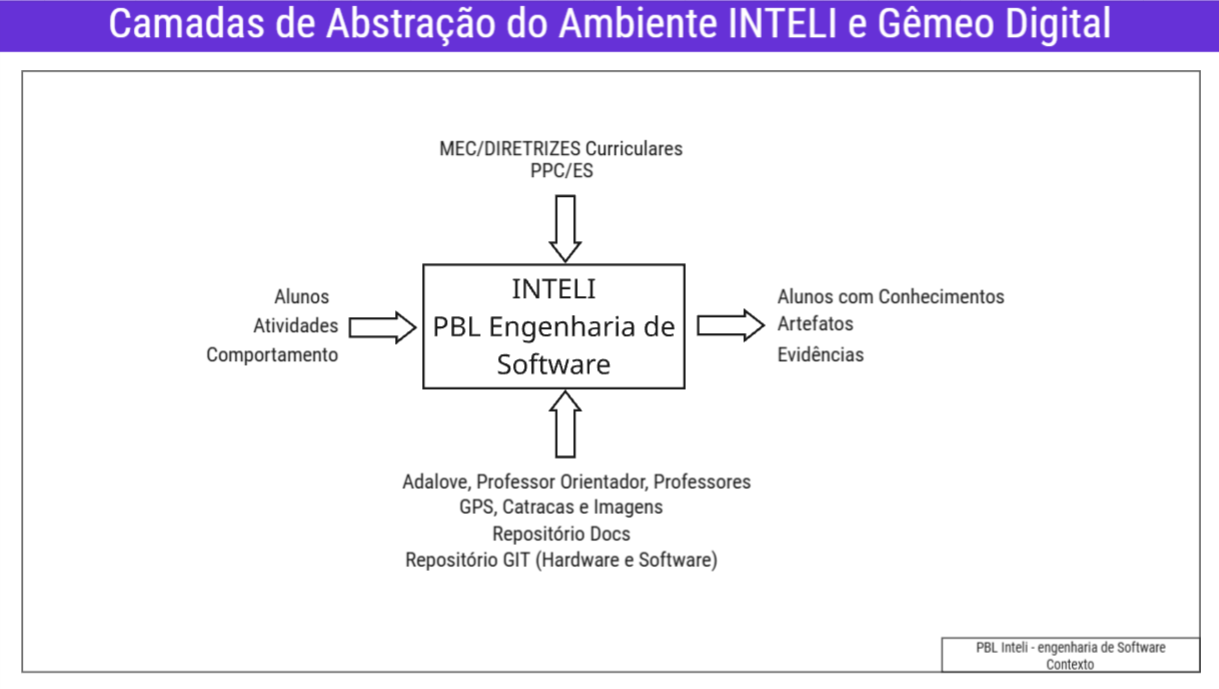
\includegraphics[scale=0.5]{assets/idf0_pbl_engsoft.png}}
	\caption{IDF0 Nível 0 - PBL em Engenharia de Software}
	\label{fig:idf0_nivel0}
\end{figure}

\subsubsection{Nível 1 - Aplicação do Módulo}

O diagrama de aplicação do módulo detalha como um módulo PBL específico é implementado, incluindo as atividades de planejamento, execução e avaliação.

\begin{figure}[h]
	\centerline{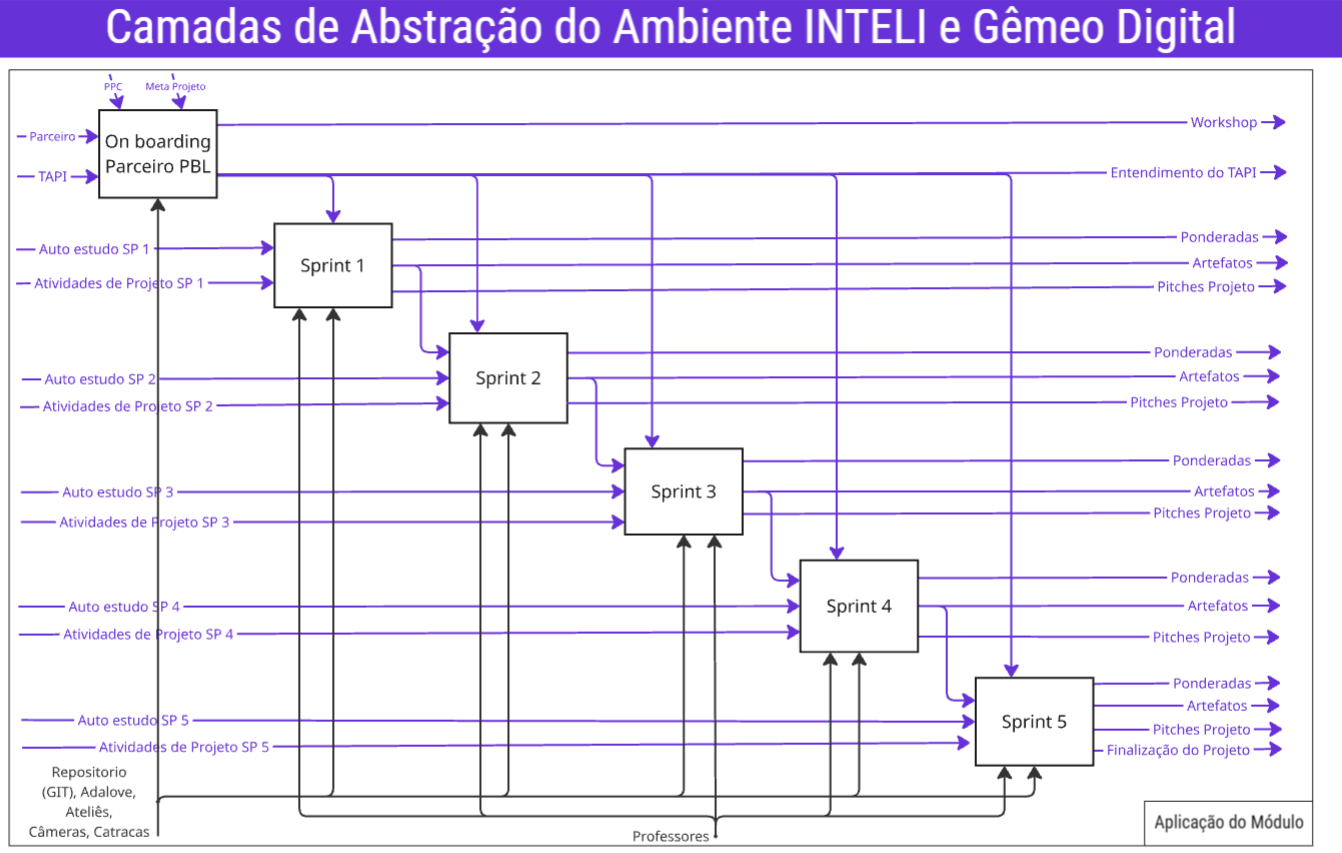
\includegraphics[scale=0.5]{assets/idf0_aplicação_módulo.png}}
	\caption{IDF0 Nível 1 - Aplicação do Módulo}
	\label{fig:idf0_nivel1}
\end{figure}

\subsubsection{Nível 2 - Sub-processos Detalhados}

O diagrama de sub-processos apresenta o detalhamento das atividades específicas dentro de cada sprint, incluindo desenvolvimento, revisão e avaliação de artefatos.

\begin{figure}[h]
	\centerline{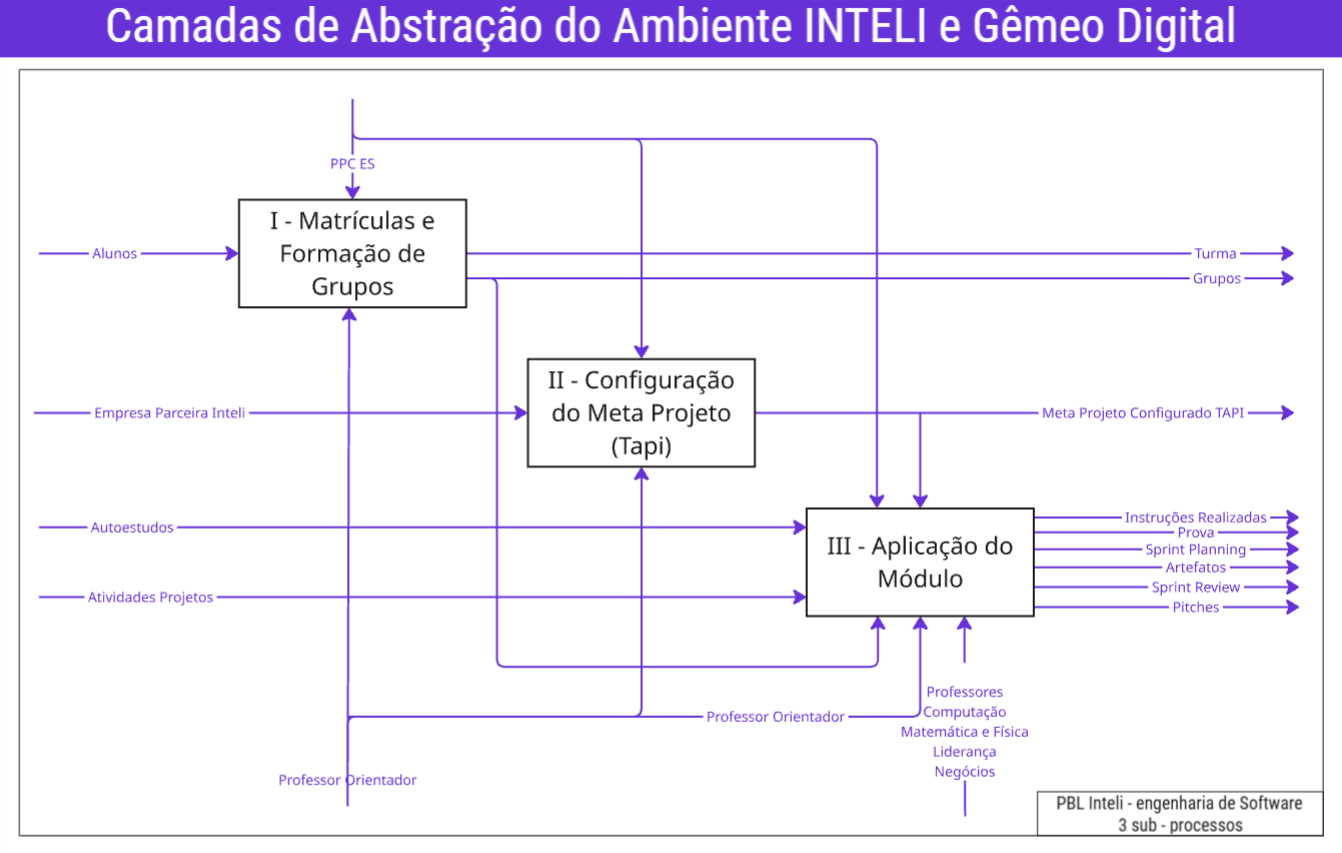
\includegraphics[scale=0.5]{assets/idf0_camada_3_sub_processos.png}}
	\caption{IDF0 Nível 2 - Sub-processos Detalhados}
	\label{fig:idf0_nivel2}
\end{figure}

\subsection{Integração das Visões}

O modelo integra as três visões arquiteturais através de mecanismos de sincronização conceitual:

\begin{itemize}
    \item \textbf{Mapeamento Entidade-Processo}: As entidades do diagrama de classes são mapeadas para as funções dos diagramas IDF0
    \item \textbf{Fluxo de Dados}: Os artefatos produzidos em cada processo são representados como instâncias das classes correspondentes
    \item \textbf{Controles e Mecanismos}: Os controles dos processos IDF0 são mapeados para os relacionamentos entre entidades
\end{itemize}

Esta integração permite que o modelo sirva como base conceitual para futuras implementações de digital twins educacionais, onde a representação virtual do sistema educacional pode ser sincronizada com o ambiente real de aprendizagem.

\section{Estudo de Caso}

[ESPAÇO RESERVADO PARA ESTUDO DE CASO FUTURO]

Esta seção será desenvolvida com base na aplicação do modelo proposto em um contexto real de PBL em engenharia de software. O estudo de caso demonstrará como o modelo arquitetural pode ser utilizado como ferramenta de suporte para docentes na avaliação de projetos educacionais.

\section{Discussão}

O modelo proposto oferece uma estrutura conceitual robusta para integração de ferramentas de avaliação em PBL de engenharia de software. A utilização de técnicas de modelagem arquitetural (IDF0 e UML) permite uma representação clara e estruturada dos processos educacionais e suas entidades.

As principais contribuições do modelo incluem:

\begin{itemize}
    \item \textbf{Estruturação Conceitual}: O modelo oferece uma estrutura clara para compreensão dos processos PBL
    \item \textbf{Integração de Visões}: A combinação de visões estrutural, comportamental e de processo permite uma compreensão holística do sistema educacional
    \item \textbf{Base para Implementação}: O modelo serve como fundamento conceitual para futuras implementações de digital twins educacionais
    \item \textbf{Suporte à Avaliação}: A estrutura proposta facilita a avaliação multidimensional de artefatos produzidos pelos estudantes
\end{itemize}

As limitações do modelo incluem:

\begin{itemize}
    \item \textbf{Natureza Conceitual}: O modelo é uma proposta conceitual que requer validação empírica
    \item \textbf{Contexto Específico}: O modelo foi desenvolvido para PBL em engenharia de software e pode não ser diretamente aplicável a outros contextos
    \item \textbf{Complexidade de Implementação}: A implementação prática do modelo requer recursos tecnológicos e de infraestrutura significativos
\end{itemize}

\section{Conclusões}

Este artigo propôs um modelo arquitetural conceitual para integração de ferramentas e processos de avaliação em PBL aplicado ao ensino de engenharia de software. O modelo utiliza técnicas de modelagem IDF0 e UML para estruturar o metaprojeto de um módulo PBL, integrando três visões arquiteturais: estrutural, comportamental e de processo.

A principal contribuição do trabalho é o preenchimento de uma lacuna identificada na literatura sobre ferramentas de suporte para docentes em PBL. O modelo oferece uma estrutura conceitual robusta que pode ser utilizada como base para futuras implementações de digital twins educacionais.

Os trabalhos futuros incluem:

\begin{itemize}
    \item Validação empírica do modelo através de estudos de caso em contextos reais de PBL
    \item Desenvolvimento de protótipos de digital twins baseados no modelo proposto
    \item Extensão do modelo para outros contextos educacionais além da engenharia de software
    \item Avaliação da eficácia do modelo como ferramenta de suporte para docentes
\end{itemize}

O modelo proposto representa um passo importante no desenvolvimento de ferramentas de suporte pedagógico para PBL, oferecendo uma base conceitual sólida para futuras pesquisas e implementações práticas.

\section*{Agradecimentos}

[ESPAÇO RESERVADO PARA AGRADECIMENTOS FUTUROS]

%====================================================================

\printbibliography
%See the guidelines for metadata and references:
%https://sol.sbc.org.br/journals/index.php/rbie/libraryFiles/downloadPublic/71
%====================================================================

\end{document}
